\section{One car, no traffic: the closed form}
\label{sec:closed}

\begin{figure*}[t]
\centering
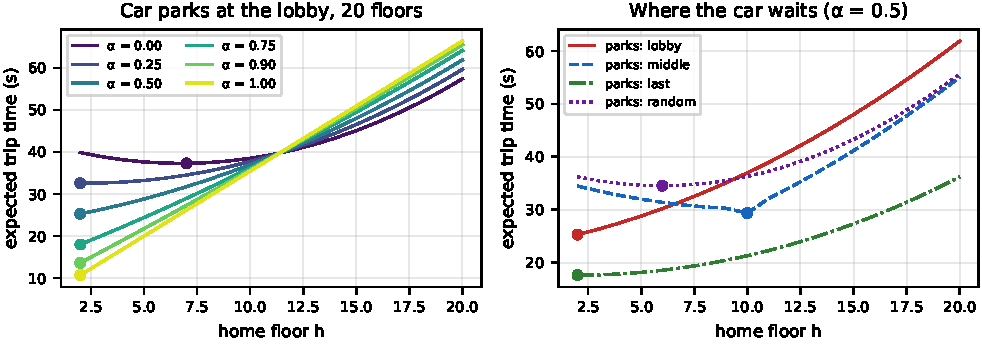
\includegraphics[width=\textwidth]{figures/curves.pdf}
\caption{Closed-form expected trip time versus home floor in a \CurveN-floor
building. Left: the car parks at the lobby; each curve is a lobby-trip
fraction $\alpha$, dots mark the optimum. Right: $\alpha = 0.5$ under the four
parking policies. The middle-floor intuition needs both no lobby trips and a
car that waits where you left it.}
\label{fig:curves}
\end{figure*}

Figure~\ref{fig:curves} is the whole argument in two panels. With no lobby
trips ($\alpha = 0$) and a car that stays where it last stopped, the wait is a
door cycle and only the ride counts: the optimum is the median floor
(\AnaMiddleLastZero\ of \CurveN) and the curve is flat around it. Change
either assumption and the optimum moves. If the car parks at the lobby, even
with $\alpha = 0$ the approach time grows with $h$ and the optimum slides to
floor \AnaLobbyZero, with an indifference band of floors
\AnaBandZeroLobby. If a quarter of trips go to the lobby, the optimum is
floor \AnaLobbyQuarter\ --- the lowest residential floor --- and it stays
there for every larger $\alpha$: at $\alpha = 0.5$ the middle floor costs
\AnaRegretMidHalfLobby\% more than the best, at $\alpha = 0.9$ it costs
\AnaRegretMidNineLobby\% more (\AnaBestNineLobby\,s versus a top floor at
\AnaWorstNineLobby\,s, \AnaRegretTopNineLobby\% worse).

The right panel isolates the mechanism. Parking at the middle floor makes the
middle floor optimal at $\alpha = 0.5$ (floor \AnaMiddleHalf), because the
approach is now shortest there; the random-position limit gives floor
\AnaRandomHalf\ with a wide band (\AnaBandZeroRandom\ at $\alpha = 0$),
because the approach no longer depends on $h$ and only the lobby trips pull
the optimum down; and the stay-put policy gives floor \AnaLastHalf\ because
the resident's own lobby trips leave the car at the lobby half the time. The
parking policy, which the resident never chooses, moves the answer as much
as the lobby fraction does. The picture scales with height: in a 40-floor
building at $\alpha = 0.5$ the optimum with lobby parking is still floor
\AnaFortyLobbyHalf\ and the middle floor's regret is
\AnaFortyRegretMidHalf\%, while the random-position, no-lobby case puts it at
floor \AnaFortyRandomZero, the median.
